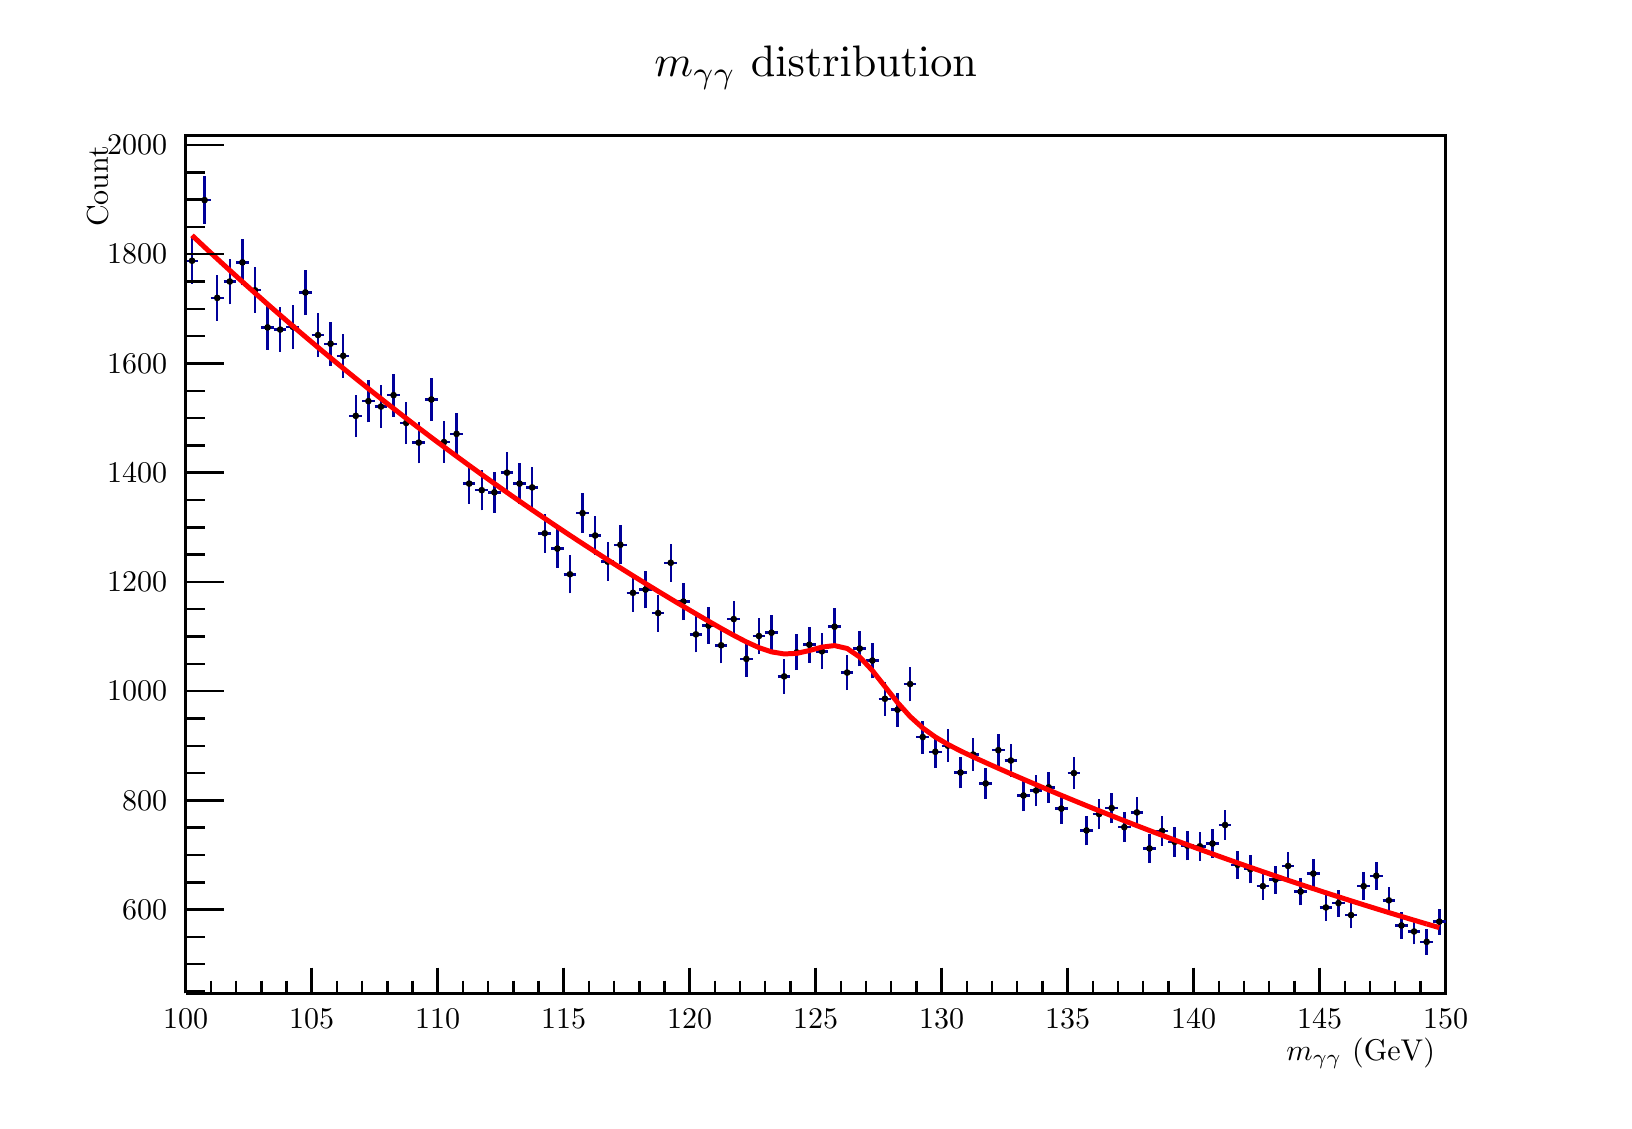
\begin{tikzpicture}
\pgfdeclareplotmark{cross} {
\pgfpathmoveto{\pgfpoint{-0.3\pgfplotmarksize}{\pgfplotmarksize}}
\pgfpathlineto{\pgfpoint{+0.3\pgfplotmarksize}{\pgfplotmarksize}}
\pgfpathlineto{\pgfpoint{+0.3\pgfplotmarksize}{0.3\pgfplotmarksize}}
\pgfpathlineto{\pgfpoint{+1\pgfplotmarksize}{0.3\pgfplotmarksize}}
\pgfpathlineto{\pgfpoint{+1\pgfplotmarksize}{-0.3\pgfplotmarksize}}
\pgfpathlineto{\pgfpoint{+0.3\pgfplotmarksize}{-0.3\pgfplotmarksize}}
\pgfpathlineto{\pgfpoint{+0.3\pgfplotmarksize}{-1.\pgfplotmarksize}}
\pgfpathlineto{\pgfpoint{-0.3\pgfplotmarksize}{-1.\pgfplotmarksize}}
\pgfpathlineto{\pgfpoint{-0.3\pgfplotmarksize}{-0.3\pgfplotmarksize}}
\pgfpathlineto{\pgfpoint{-1.\pgfplotmarksize}{-0.3\pgfplotmarksize}}
\pgfpathlineto{\pgfpoint{-1.\pgfplotmarksize}{0.3\pgfplotmarksize}}
\pgfpathlineto{\pgfpoint{-0.3\pgfplotmarksize}{0.3\pgfplotmarksize}}
\pgfpathclose
\pgfusepathqstroke
}
\pgfdeclareplotmark{cross*} {
\pgfpathmoveto{\pgfpoint{-0.3\pgfplotmarksize}{\pgfplotmarksize}}
\pgfpathlineto{\pgfpoint{+0.3\pgfplotmarksize}{\pgfplotmarksize}}
\pgfpathlineto{\pgfpoint{+0.3\pgfplotmarksize}{0.3\pgfplotmarksize}}
\pgfpathlineto{\pgfpoint{+1\pgfplotmarksize}{0.3\pgfplotmarksize}}
\pgfpathlineto{\pgfpoint{+1\pgfplotmarksize}{-0.3\pgfplotmarksize}}
\pgfpathlineto{\pgfpoint{+0.3\pgfplotmarksize}{-0.3\pgfplotmarksize}}
\pgfpathlineto{\pgfpoint{+0.3\pgfplotmarksize}{-1.\pgfplotmarksize}}
\pgfpathlineto{\pgfpoint{-0.3\pgfplotmarksize}{-1.\pgfplotmarksize}}
\pgfpathlineto{\pgfpoint{-0.3\pgfplotmarksize}{-0.3\pgfplotmarksize}}
\pgfpathlineto{\pgfpoint{-1.\pgfplotmarksize}{-0.3\pgfplotmarksize}}
\pgfpathlineto{\pgfpoint{-1.\pgfplotmarksize}{0.3\pgfplotmarksize}}
\pgfpathlineto{\pgfpoint{-0.3\pgfplotmarksize}{0.3\pgfplotmarksize}}
\pgfpathclose
\pgfusepathqfillstroke
}
\pgfdeclareplotmark{newstar} {
\pgfpathmoveto{\pgfqpoint{0pt}{\pgfplotmarksize}}
\pgfpathlineto{\pgfqpointpolar{44}{0.5\pgfplotmarksize}}
\pgfpathlineto{\pgfqpointpolar{18}{\pgfplotmarksize}}
\pgfpathlineto{\pgfqpointpolar{-20}{0.5\pgfplotmarksize}}
\pgfpathlineto{\pgfqpointpolar{-54}{\pgfplotmarksize}}
\pgfpathlineto{\pgfqpointpolar{-90}{0.5\pgfplotmarksize}}
\pgfpathlineto{\pgfqpointpolar{234}{\pgfplotmarksize}}
\pgfpathlineto{\pgfqpointpolar{198}{0.5\pgfplotmarksize}}
\pgfpathlineto{\pgfqpointpolar{162}{\pgfplotmarksize}}
\pgfpathlineto{\pgfqpointpolar{134}{0.5\pgfplotmarksize}}
\pgfpathclose
\pgfusepathqstroke
}
\pgfdeclareplotmark{newstar*} {
\pgfpathmoveto{\pgfqpoint{0pt}{\pgfplotmarksize}}
\pgfpathlineto{\pgfqpointpolar{44}{0.5\pgfplotmarksize}}
\pgfpathlineto{\pgfqpointpolar{18}{\pgfplotmarksize}}
\pgfpathlineto{\pgfqpointpolar{-20}{0.5\pgfplotmarksize}}
\pgfpathlineto{\pgfqpointpolar{-54}{\pgfplotmarksize}}
\pgfpathlineto{\pgfqpointpolar{-90}{0.5\pgfplotmarksize}}
\pgfpathlineto{\pgfqpointpolar{234}{\pgfplotmarksize}}
\pgfpathlineto{\pgfqpointpolar{198}{0.5\pgfplotmarksize}}
\pgfpathlineto{\pgfqpointpolar{162}{\pgfplotmarksize}}
\pgfpathlineto{\pgfqpointpolar{134}{0.5\pgfplotmarksize}}
\pgfpathclose
\pgfusepathqfillstroke
}
\definecolor{c}{rgb}{1,1,1};
\draw [color=c, fill=c] (0,0) rectangle (20,13.6207);
\draw [color=c, fill=c] (2,1.36207) rectangle (18,12.2586);
\definecolor{c}{rgb}{0,0,0};
\draw [c,line width=0.9] (2,1.36207) -- (2,12.2586) -- (18,12.2586) -- (18,1.36207) -- (2,1.36207);
\definecolor{c}{rgb}{1,1,1};
\draw [color=c, fill=c] (2,1.36207) rectangle (18,12.2586);
\definecolor{c}{rgb}{0,0,0};
\draw [c,line width=0.9] (2,1.36207) -- (2,12.2586) -- (18,12.2586) -- (18,1.36207) -- (2,1.36207);
\definecolor{c}{rgb}{0,0,0.6};
\draw [c,line width=0.9] (2.08,10.3742) -- (2.08,10.6675);
\draw [c,line width=0.9] (2.08,10.6675) -- (2.08,10.9608);
\draw [c,line width=0.9] (2,10.6675) -- (2.08,10.6675);
\draw [c,line width=0.9] (2.08,10.6675) -- (2.16,10.6675);
\definecolor{c}{rgb}{0,0,0};
\foreach \P in {(2.08,10.6675)}{\draw[mark options={color=c,fill=c},mark size=2.402402pt,mark=*,mark size=1pt] plot coordinates {\P};}
\definecolor{c}{rgb}{0,0,0.6};
\draw [c,line width=0.9] (2.24,11.1352) -- (2.24,11.4375);
\draw [c,line width=0.9] (2.24,11.4375) -- (2.24,11.7397);
\draw [c,line width=0.9] (2.16,11.4375) -- (2.24,11.4375);
\draw [c,line width=0.9] (2.24,11.4375) -- (2.32,11.4375);
\definecolor{c}{rgb}{0,0,0};
\foreach \P in {(2.24,11.4375)}{\draw[mark options={color=c,fill=c},mark size=2.402402pt,mark=*,mark size=1pt] plot coordinates {\P};}
\definecolor{c}{rgb}{0,0,0.6};
\draw [c,line width=0.9] (2.4,9.90813) -- (2.4,10.1958);
\draw [c,line width=0.9] (2.4,10.1958) -- (2.4,10.4835);
\draw [c,line width=0.9] (2.32,10.1958) -- (2.4,10.1958);
\draw [c,line width=0.9] (2.4,10.1958) -- (2.48,10.1958);
\definecolor{c}{rgb}{0,0,0};
\foreach \P in {(2.4,10.1958)}{\draw[mark options={color=c,fill=c},mark size=2.402402pt,mark=*,mark size=1pt] plot coordinates {\P};}
\definecolor{c}{rgb}{0,0,0.6};
\draw [c,line width=0.9] (2.56,10.1137) -- (2.56,10.4039);
\draw [c,line width=0.9] (2.56,10.4039) -- (2.56,10.6941);
\draw [c,line width=0.9] (2.48,10.4039) -- (2.56,10.4039);
\draw [c,line width=0.9] (2.56,10.4039) -- (2.64,10.4039);
\definecolor{c}{rgb}{0,0,0};
\foreach \P in {(2.56,10.4039)}{\draw[mark options={color=c,fill=c},mark size=2.402402pt,mark=*,mark size=1pt] plot coordinates {\P};}
\definecolor{c}{rgb}{0,0,0.6};
\draw [c,line width=0.9] (2.72,10.3536) -- (2.72,10.6467);
\draw [c,line width=0.9] (2.72,10.6467) -- (2.72,10.9398);
\draw [c,line width=0.9] (2.64,10.6467) -- (2.72,10.6467);
\draw [c,line width=0.9] (2.72,10.6467) -- (2.8,10.6467);
\definecolor{c}{rgb}{0,0,0};
\foreach \P in {(2.72,10.6467)}{\draw[mark options={color=c,fill=c},mark size=2.402402pt,mark=*,mark size=1pt] plot coordinates {\P};}
\definecolor{c}{rgb}{0,0,0.6};
\draw [c,line width=0.9] (2.88,10.0041) -- (2.88,10.2929);
\draw [c,line width=0.9] (2.88,10.2929) -- (2.88,10.5818);
\draw [c,line width=0.9] (2.8,10.2929) -- (2.88,10.2929);
\draw [c,line width=0.9] (2.88,10.2929) -- (2.96,10.2929);
\definecolor{c}{rgb}{0,0,0};
\foreach \P in {(2.88,10.2929)}{\draw[mark options={color=c,fill=c},mark size=2.402402pt,mark=*,mark size=1pt] plot coordinates {\P};}
\definecolor{c}{rgb}{0,0,0.6};
\draw [c,line width=0.9] (3.04,9.53811) -- (3.04,9.82124);
\draw [c,line width=0.9] (3.04,9.82124) -- (3.04,10.1044);
\draw [c,line width=0.9] (2.96,9.82124) -- (3.04,9.82124);
\draw [c,line width=0.9] (3.04,9.82124) -- (3.12,9.82124);
\definecolor{c}{rgb}{0,0,0};
\foreach \P in {(3.04,9.82124)}{\draw[mark options={color=c,fill=c},mark size=2.402402pt,mark=*,mark size=1pt] plot coordinates {\P};}
\definecolor{c}{rgb}{0,0,0.6};
\draw [c,line width=0.9] (3.2,9.5107) -- (3.2,9.79349);
\draw [c,line width=0.9] (3.2,9.79349) -- (3.2,10.0763);
\draw [c,line width=0.9] (3.12,9.79349) -- (3.2,9.79349);
\draw [c,line width=0.9] (3.2,9.79349) -- (3.28,9.79349);
\definecolor{c}{rgb}{0,0,0};
\foreach \P in {(3.2,9.79349)}{\draw[mark options={color=c,fill=c},mark size=2.402402pt,mark=*,mark size=1pt] plot coordinates {\P};}
\definecolor{c}{rgb}{0,0,0.6};
\draw [c,line width=0.9] (3.36,9.54496) -- (3.36,9.82817);
\draw [c,line width=0.9] (3.36,9.82817) -- (3.36,10.1114);
\draw [c,line width=0.9] (3.28,9.82817) -- (3.36,9.82817);
\draw [c,line width=0.9] (3.36,9.82817) -- (3.44,9.82817);
\definecolor{c}{rgb}{0,0,0};
\foreach \P in {(3.36,9.82817)}{\draw[mark options={color=c,fill=c},mark size=2.402402pt,mark=*,mark size=1pt] plot coordinates {\P};}
\definecolor{c}{rgb}{0,0,0.6};
\draw [c,line width=0.9] (3.52,9.97666) -- (3.52,10.2652);
\draw [c,line width=0.9] (3.52,10.2652) -- (3.52,10.5537);
\draw [c,line width=0.9] (3.44,10.2652) -- (3.52,10.2652);
\draw [c,line width=0.9] (3.52,10.2652) -- (3.6,10.2652);
\definecolor{c}{rgb}{0,0,0};
\foreach \P in {(3.52,10.2652)}{\draw[mark options={color=c,fill=c},mark size=2.402402pt,mark=*,mark size=1pt] plot coordinates {\P};}
\definecolor{c}{rgb}{0,0,0.6};
\draw [c,line width=0.9] (3.68,9.44219) -- (3.68,9.72412);
\draw [c,line width=0.9] (3.68,9.72412) -- (3.68,10.0061);
\draw [c,line width=0.9] (3.6,9.72412) -- (3.68,9.72412);
\draw [c,line width=0.9] (3.68,9.72412) -- (3.76,9.72412);
\definecolor{c}{rgb}{0,0,0};
\foreach \P in {(3.68,9.72412)}{\draw[mark options={color=c,fill=c},mark size=2.402402pt,mark=*,mark size=1pt] plot coordinates {\P};}
\definecolor{c}{rgb}{0,0,0.6};
\draw [c,line width=0.9] (3.84,9.33257) -- (3.84,9.61314);
\draw [c,line width=0.9] (3.84,9.61314) -- (3.84,9.89371);
\draw [c,line width=0.9] (3.76,9.61314) -- (3.84,9.61314);
\draw [c,line width=0.9] (3.84,9.61314) -- (3.92,9.61314);
\definecolor{c}{rgb}{0,0,0};
\foreach \P in {(3.84,9.61314)}{\draw[mark options={color=c,fill=c},mark size=2.402402pt,mark=*,mark size=1pt] plot coordinates {\P};}
\definecolor{c}{rgb}{0,0,0.6};
\draw [c,line width=0.9] (4,9.18186) -- (4,9.46053);
\draw [c,line width=0.9] (4,9.46053) -- (4,9.73921);
\draw [c,line width=0.9] (3.92,9.46053) -- (4,9.46053);
\draw [c,line width=0.9] (4,9.46053) -- (4.08,9.46053);
\definecolor{c}{rgb}{0,0,0};
\foreach \P in {(4,9.46053)}{\draw[mark options={color=c,fill=c},mark size=2.402402pt,mark=*,mark size=1pt] plot coordinates {\P};}
\definecolor{c}{rgb}{0,0,0.6};
\draw [c,line width=0.9] (4.16,8.4285) -- (4.16,8.69751);
\draw [c,line width=0.9] (4.16,8.69751) -- (4.16,8.96652);
\draw [c,line width=0.9] (4.08,8.69751) -- (4.16,8.69751);
\draw [c,line width=0.9] (4.16,8.69751) -- (4.24,8.69751);
\definecolor{c}{rgb}{0,0,0};
\foreach \P in {(4.16,8.69751)}{\draw[mark options={color=c,fill=c},mark size=2.402402pt,mark=*,mark size=1pt] plot coordinates {\P};}
\definecolor{c}{rgb}{0,0,0.6};
\draw [c,line width=0.9] (4.32,8.61338) -- (4.32,8.8848);
\draw [c,line width=0.9] (4.32,8.8848) -- (4.32,9.15621);
\draw [c,line width=0.9] (4.24,8.8848) -- (4.32,8.8848);
\draw [c,line width=0.9] (4.32,8.8848) -- (4.4,8.8848);
\definecolor{c}{rgb}{0,0,0};
\foreach \P in {(4.32,8.8848)}{\draw[mark options={color=c,fill=c},mark size=2.402402pt,mark=*,mark size=1pt] plot coordinates {\P};}
\definecolor{c}{rgb}{0,0,0.6};
\draw [c,line width=0.9] (4.48,8.5449) -- (4.48,8.81543);
\draw [c,line width=0.9] (4.48,8.81543) -- (4.48,9.08596);
\draw [c,line width=0.9] (4.4,8.81543) -- (4.48,8.81543);
\draw [c,line width=0.9] (4.48,8.81543) -- (4.56,8.81543);
\definecolor{c}{rgb}{0,0,0};
\foreach \P in {(4.48,8.81543)}{\draw[mark options={color=c,fill=c},mark size=2.402402pt,mark=*,mark size=1pt] plot coordinates {\P};}
\definecolor{c}{rgb}{0,0,0.6};
\draw [c,line width=0.9] (4.64,8.68871) -- (4.64,8.9611);
\draw [c,line width=0.9] (4.64,8.9611) -- (4.64,9.23349);
\draw [c,line width=0.9] (4.56,8.9611) -- (4.64,8.9611);
\draw [c,line width=0.9] (4.64,8.9611) -- (4.72,8.9611);
\definecolor{c}{rgb}{0,0,0};
\foreach \P in {(4.64,8.9611)}{\draw[mark options={color=c,fill=c},mark size=2.402402pt,mark=*,mark size=1pt] plot coordinates {\P};}
\definecolor{c}{rgb}{0,0,0.6};
\draw [c,line width=0.9] (4.8,8.33949) -- (4.8,8.60733);
\draw [c,line width=0.9] (4.8,8.60733) -- (4.8,8.87518);
\draw [c,line width=0.9] (4.72,8.60733) -- (4.8,8.60733);
\draw [c,line width=0.9] (4.8,8.60733) -- (4.88,8.60733);
\definecolor{c}{rgb}{0,0,0};
\foreach \P in {(4.8,8.60733)}{\draw[mark options={color=c,fill=c},mark size=2.402402pt,mark=*,mark size=1pt] plot coordinates {\P};}
\definecolor{c}{rgb}{0,0,0.6};
\draw [c,line width=0.9] (4.96,8.09303) -- (4.96,8.35762);
\draw [c,line width=0.9] (4.96,8.35762) -- (4.96,8.62221);
\draw [c,line width=0.9] (4.88,8.35762) -- (4.96,8.35762);
\draw [c,line width=0.9] (4.96,8.35762) -- (5.04,8.35762);
\definecolor{c}{rgb}{0,0,0};
\foreach \P in {(4.96,8.35762)}{\draw[mark options={color=c,fill=c},mark size=2.402402pt,mark=*,mark size=1pt] plot coordinates {\P};}
\definecolor{c}{rgb}{0,0,0.6};
\draw [c,line width=0.9] (5.12,8.63393) -- (5.12,8.90561);
\draw [c,line width=0.9] (5.12,8.90561) -- (5.12,9.17729);
\draw [c,line width=0.9] (5.04,8.90561) -- (5.12,8.90561);
\draw [c,line width=0.9] (5.12,8.90561) -- (5.2,8.90561);
\definecolor{c}{rgb}{0,0,0};
\foreach \P in {(5.12,8.90561)}{\draw[mark options={color=c,fill=c},mark size=2.402402pt,mark=*,mark size=1pt] plot coordinates {\P};}
\definecolor{c}{rgb}{0,0,0.6};
\draw [c,line width=0.9] (5.28,8.09987) -- (5.28,8.36455);
\draw [c,line width=0.9] (5.28,8.36455) -- (5.28,8.62924);
\draw [c,line width=0.9] (5.2,8.36455) -- (5.28,8.36455);
\draw [c,line width=0.9] (5.28,8.36455) -- (5.36,8.36455);
\definecolor{c}{rgb}{0,0,0};
\foreach \P in {(5.28,8.36455)}{\draw[mark options={color=c,fill=c},mark size=2.402402pt,mark=*,mark size=1pt] plot coordinates {\P};}
\definecolor{c}{rgb}{0,0,0.6};
\draw [c,line width=0.9] (5.44,8.20256) -- (5.44,8.4686);
\draw [c,line width=0.9] (5.44,8.4686) -- (5.44,8.73464);
\draw [c,line width=0.9] (5.36,8.4686) -- (5.44,8.4686);
\draw [c,line width=0.9] (5.44,8.4686) -- (5.52,8.4686);
\definecolor{c}{rgb}{0,0,0};
\foreach \P in {(5.44,8.4686)}{\draw[mark options={color=c,fill=c},mark size=2.402402pt,mark=*,mark size=1pt] plot coordinates {\P};}
\definecolor{c}{rgb}{0,0,0.6};
\draw [c,line width=0.9] (5.6,7.57969) -- (5.6,7.83737);
\draw [c,line width=0.9] (5.6,7.83737) -- (5.6,8.09506);
\draw [c,line width=0.9] (5.52,7.83737) -- (5.6,7.83737);
\draw [c,line width=0.9] (5.6,7.83737) -- (5.68,7.83737);
\definecolor{c}{rgb}{0,0,0};
\foreach \P in {(5.6,7.83737)}{\draw[mark options={color=c,fill=c},mark size=2.402402pt,mark=*,mark size=1pt] plot coordinates {\P};}
\definecolor{c}{rgb}{0,0,0.6};
\draw [c,line width=0.9] (5.76,7.49758) -- (5.76,7.75413);
\draw [c,line width=0.9] (5.76,7.75413) -- (5.76,8.01069);
\draw [c,line width=0.9] (5.68,7.75413) -- (5.76,7.75413);
\draw [c,line width=0.9] (5.76,7.75413) -- (5.84,7.75413);
\definecolor{c}{rgb}{0,0,0};
\foreach \P in {(5.76,7.75413)}{\draw[mark options={color=c,fill=c},mark size=2.402402pt,mark=*,mark size=1pt] plot coordinates {\P};}
\definecolor{c}{rgb}{0,0,0.6};
\draw [c,line width=0.9] (5.92,7.4702) -- (5.92,7.72639);
\draw [c,line width=0.9] (5.92,7.72639) -- (5.92,7.98257);
\draw [c,line width=0.9] (5.84,7.72639) -- (5.92,7.72639);
\draw [c,line width=0.9] (5.92,7.72639) -- (6,7.72639);
\definecolor{c}{rgb}{0,0,0};
\foreach \P in {(5.92,7.72639)}{\draw[mark options={color=c,fill=c},mark size=2.402402pt,mark=*,mark size=1pt] plot coordinates {\P};}
\definecolor{c}{rgb}{0,0,0.6};
\draw [c,line width=0.9] (6.08,7.71656) -- (6.08,7.97611);
\draw [c,line width=0.9] (6.08,7.97611) -- (6.08,8.23565);
\draw [c,line width=0.9] (6,7.97611) -- (6.08,7.97611);
\draw [c,line width=0.9] (6.08,7.97611) -- (6.16,7.97611);
\definecolor{c}{rgb}{0,0,0};
\foreach \P in {(6.08,7.97611)}{\draw[mark options={color=c,fill=c},mark size=2.402402pt,mark=*,mark size=1pt] plot coordinates {\P};}
\definecolor{c}{rgb}{0,0,0.6};
\draw [c,line width=0.9] (6.24,7.57969) -- (6.24,7.83737);
\draw [c,line width=0.9] (6.24,7.83737) -- (6.24,8.09506);
\draw [c,line width=0.9] (6.16,7.83737) -- (6.24,7.83737);
\draw [c,line width=0.9] (6.24,7.83737) -- (6.32,7.83737);
\definecolor{c}{rgb}{0,0,0};
\foreach \P in {(6.24,7.83737)}{\draw[mark options={color=c,fill=c},mark size=2.402402pt,mark=*,mark size=1pt] plot coordinates {\P};}
\definecolor{c}{rgb}{0,0,0.6};
\draw [c,line width=0.9] (6.4,7.53179) -- (6.4,7.78882);
\draw [c,line width=0.9] (6.4,7.78882) -- (6.4,8.04585);
\draw [c,line width=0.9] (6.32,7.78882) -- (6.4,7.78882);
\draw [c,line width=0.9] (6.4,7.78882) -- (6.48,7.78882);
\definecolor{c}{rgb}{0,0,0};
\foreach \P in {(6.4,7.78882)}{\draw[mark options={color=c,fill=c},mark size=2.402402pt,mark=*,mark size=1pt] plot coordinates {\P};}
\definecolor{c}{rgb}{0,0,0.6};
\draw [c,line width=0.9] (6.56,6.9571) -- (6.56,7.20615);
\draw [c,line width=0.9] (6.56,7.20615) -- (6.56,7.45519);
\draw [c,line width=0.9] (6.48,7.20615) -- (6.56,7.20615);
\draw [c,line width=0.9] (6.56,7.20615) -- (6.64,7.20615);
\definecolor{c}{rgb}{0,0,0};
\foreach \P in {(6.56,7.20615)}{\draw[mark options={color=c,fill=c},mark size=2.402402pt,mark=*,mark size=1pt] plot coordinates {\P};}
\definecolor{c}{rgb}{0,0,0.6};
\draw [c,line width=0.9] (6.72,6.7656) -- (6.72,7.01192);
\draw [c,line width=0.9] (6.72,7.01192) -- (6.72,7.25824);
\draw [c,line width=0.9] (6.64,7.01192) -- (6.72,7.01192);
\draw [c,line width=0.9] (6.72,7.01192) -- (6.8,7.01192);
\definecolor{c}{rgb}{0,0,0};
\foreach \P in {(6.72,7.01192)}{\draw[mark options={color=c,fill=c},mark size=2.402402pt,mark=*,mark size=1pt] plot coordinates {\P};}
\definecolor{c}{rgb}{0,0,0.6};
\draw [c,line width=0.9] (6.88,6.44421) -- (6.88,6.6859);
\draw [c,line width=0.9] (6.88,6.6859) -- (6.88,6.92759);
\draw [c,line width=0.9] (6.8,6.6859) -- (6.88,6.6859);
\draw [c,line width=0.9] (6.88,6.6859) -- (6.96,6.6859);
\definecolor{c}{rgb}{0,0,0};
\foreach \P in {(6.88,6.6859)}{\draw[mark options={color=c,fill=c},mark size=2.402402pt,mark=*,mark size=1pt] plot coordinates {\P};}
\definecolor{c}{rgb}{0,0,0.6};
\draw [c,line width=0.9] (7.04,7.21021) -- (7.04,7.4628);
\draw [c,line width=0.9] (7.04,7.4628) -- (7.04,7.71539);
\draw [c,line width=0.9] (6.96,7.4628) -- (7.04,7.4628);
\draw [c,line width=0.9] (7.04,7.4628) -- (7.12,7.4628);
\definecolor{c}{rgb}{0,0,0};
\foreach \P in {(7.04,7.4628)}{\draw[mark options={color=c,fill=c},mark size=2.402402pt,mark=*,mark size=1pt] plot coordinates {\P};}
\definecolor{c}{rgb}{0,0,0.6};
\draw [c,line width=0.9] (7.2,6.92974) -- (7.2,7.1784);
\draw [c,line width=0.9] (7.2,7.1784) -- (7.2,7.42705);
\draw [c,line width=0.9] (7.12,7.1784) -- (7.2,7.1784);
\draw [c,line width=0.9] (7.2,7.1784) -- (7.28,7.1784);
\definecolor{c}{rgb}{0,0,0};
\foreach \P in {(7.2,7.1784)}{\draw[mark options={color=c,fill=c},mark size=2.402402pt,mark=*,mark size=1pt] plot coordinates {\P};}
\definecolor{c}{rgb}{0,0,0.6};
\draw [c,line width=0.9] (7.36,6.60148) -- (7.36,6.84544);
\draw [c,line width=0.9] (7.36,6.84544) -- (7.36,7.08941);
\draw [c,line width=0.9] (7.28,6.84544) -- (7.36,6.84544);
\draw [c,line width=0.9] (7.36,6.84544) -- (7.44,6.84544);
\definecolor{c}{rgb}{0,0,0};
\foreach \P in {(7.36,6.84544)}{\draw[mark options={color=c,fill=c},mark size=2.402402pt,mark=*,mark size=1pt] plot coordinates {\P};}
\definecolor{c}{rgb}{0,0,0.6};
\draw [c,line width=0.9] (7.52,6.81347) -- (7.52,7.06048);
\draw [c,line width=0.9] (7.52,7.06048) -- (7.52,7.30748);
\draw [c,line width=0.9] (7.44,7.06048) -- (7.52,7.06048);
\draw [c,line width=0.9] (7.52,7.06048) -- (7.6,7.06048);
\definecolor{c}{rgb}{0,0,0};
\foreach \P in {(7.52,7.06048)}{\draw[mark options={color=c,fill=c},mark size=2.402402pt,mark=*,mark size=1pt] plot coordinates {\P};}
\definecolor{c}{rgb}{0,0,0.6};
\draw [c,line width=0.9] (7.68,6.21178) -- (7.68,6.45006);
\draw [c,line width=0.9] (7.68,6.45006) -- (7.68,6.68834);
\draw [c,line width=0.9] (7.6,6.45006) -- (7.68,6.45006);
\draw [c,line width=0.9] (7.68,6.45006) -- (7.76,6.45006);
\definecolor{c}{rgb}{0,0,0};
\foreach \P in {(7.68,6.45006)}{\draw[mark options={color=c,fill=c},mark size=2.402402pt,mark=*,mark size=1pt] plot coordinates {\P};}
\definecolor{c}{rgb}{0,0,0.6};
\draw [c,line width=0.9] (7.84,6.25279) -- (7.84,6.49168);
\draw [c,line width=0.9] (7.84,6.49168) -- (7.84,6.73056);
\draw [c,line width=0.9] (7.76,6.49168) -- (7.84,6.49168);
\draw [c,line width=0.9] (7.84,6.49168) -- (7.92,6.49168);
\definecolor{c}{rgb}{0,0,0};
\foreach \P in {(7.84,6.49168)}{\draw[mark options={color=c,fill=c},mark size=2.402402pt,mark=*,mark size=1pt] plot coordinates {\P};}
\definecolor{c}{rgb}{0,0,0.6};
\draw [c,line width=0.9] (8,5.95889) -- (8,6.1934);
\draw [c,line width=0.9] (8,6.1934) -- (8,6.42792);
\draw [c,line width=0.9] (7.92,6.1934) -- (8,6.1934);
\draw [c,line width=0.9] (8,6.1934) -- (8.08,6.1934);
\definecolor{c}{rgb}{0,0,0};
\foreach \P in {(8,6.1934)}{\draw[mark options={color=c,fill=c},mark size=2.402402pt,mark=*,mark size=1pt] plot coordinates {\P};}
\definecolor{c}{rgb}{0,0,0.6};
\draw [c,line width=0.9] (8.16,6.5878) -- (8.16,6.83157);
\draw [c,line width=0.9] (8.16,6.83157) -- (8.16,7.07534);
\draw [c,line width=0.9] (8.08,6.83157) -- (8.16,6.83157);
\draw [c,line width=0.9] (8.16,6.83157) -- (8.24,6.83157);
\definecolor{c}{rgb}{0,0,0};
\foreach \P in {(8.16,6.83157)}{\draw[mark options={color=c,fill=c},mark size=2.402402pt,mark=*,mark size=1pt] plot coordinates {\P};}
\definecolor{c}{rgb}{0,0,0.6};
\draw [c,line width=0.9] (8.32,6.10241) -- (8.32,6.33907);
\draw [c,line width=0.9] (8.32,6.33907) -- (8.32,6.57573);
\draw [c,line width=0.9] (8.24,6.33907) -- (8.32,6.33907);
\draw [c,line width=0.9] (8.32,6.33907) -- (8.4,6.33907);
\definecolor{c}{rgb}{0,0,0};
\foreach \P in {(8.32,6.33907)}{\draw[mark options={color=c,fill=c},mark size=2.402402pt,mark=*,mark size=1pt] plot coordinates {\P};}
\definecolor{c}{rgb}{0,0,0.6};
\draw [c,line width=0.9] (8.48,5.6924) -- (8.48,5.92288);
\draw [c,line width=0.9] (8.48,5.92288) -- (8.48,6.15336);
\draw [c,line width=0.9] (8.4,5.92288) -- (8.48,5.92288);
\draw [c,line width=0.9] (8.48,5.92288) -- (8.56,5.92288);
\definecolor{c}{rgb}{0,0,0};
\foreach \P in {(8.48,5.92288)}{\draw[mark options={color=c,fill=c},mark size=2.402402pt,mark=*,mark size=1pt] plot coordinates {\P};}
\definecolor{c}{rgb}{0,0,0.6};
\draw [c,line width=0.9] (8.64,5.80172) -- (8.64,6.03386);
\draw [c,line width=0.9] (8.64,6.03386) -- (8.64,6.26601);
\draw [c,line width=0.9] (8.56,6.03386) -- (8.64,6.03386);
\draw [c,line width=0.9] (8.64,6.03386) -- (8.72,6.03386);
\definecolor{c}{rgb}{0,0,0};
\foreach \P in {(8.64,6.03386)}{\draw[mark options={color=c,fill=c},mark size=2.402402pt,mark=*,mark size=1pt] plot coordinates {\P};}
\definecolor{c}{rgb}{0,0,0.6};
\draw [c,line width=0.9] (8.8,5.55577) -- (8.8,5.78415);
\draw [c,line width=0.9] (8.8,5.78415) -- (8.8,6.01253);
\draw [c,line width=0.9] (8.72,5.78415) -- (8.8,5.78415);
\draw [c,line width=0.9] (8.8,5.78415) -- (8.88,5.78415);
\definecolor{c}{rgb}{0,0,0};
\foreach \P in {(8.8,5.78415)}{\draw[mark options={color=c,fill=c},mark size=2.402402pt,mark=*,mark size=1pt] plot coordinates {\P};}
\definecolor{c}{rgb}{0,0,0.6};
\draw [c,line width=0.9] (8.96,5.88372) -- (8.96,6.1171);
\draw [c,line width=0.9] (8.96,6.1171) -- (8.96,6.35048);
\draw [c,line width=0.9] (8.88,6.1171) -- (8.96,6.1171);
\draw [c,line width=0.9] (8.96,6.1171) -- (9.04,6.1171);
\definecolor{c}{rgb}{0,0,0};
\foreach \P in {(8.96,6.1171)}{\draw[mark options={color=c,fill=c},mark size=2.402402pt,mark=*,mark size=1pt] plot coordinates {\P};}
\definecolor{c}{rgb}{0,0,0.6};
\draw [c,line width=0.9] (9.12,5.385) -- (9.12,5.61073);
\draw [c,line width=0.9] (9.12,5.61073) -- (9.12,5.83646);
\draw [c,line width=0.9] (9.04,5.61073) -- (9.12,5.61073);
\draw [c,line width=0.9] (9.12,5.61073) -- (9.2,5.61073);
\definecolor{c}{rgb}{0,0,0};
\foreach \P in {(9.12,5.61073)}{\draw[mark options={color=c,fill=c},mark size=2.402402pt,mark=*,mark size=1pt] plot coordinates {\P};}
\definecolor{c}{rgb}{0,0,0.6};
\draw [c,line width=0.9] (9.28,5.6719) -- (9.28,5.90207);
\draw [c,line width=0.9] (9.28,5.90207) -- (9.28,6.13223);
\draw [c,line width=0.9] (9.2,5.90207) -- (9.28,5.90207);
\draw [c,line width=0.9] (9.28,5.90207) -- (9.36,5.90207);
\definecolor{c}{rgb}{0,0,0};
\foreach \P in {(9.28,5.90207)}{\draw[mark options={color=c,fill=c},mark size=2.402402pt,mark=*,mark size=1pt] plot coordinates {\P};}
\definecolor{c}{rgb}{0,0,0.6};
\draw [c,line width=0.9] (9.44,5.7129) -- (9.44,5.94369);
\draw [c,line width=0.9] (9.44,5.94369) -- (9.44,6.17448);
\draw [c,line width=0.9] (9.36,5.94369) -- (9.44,5.94369);
\draw [c,line width=0.9] (9.44,5.94369) -- (9.52,5.94369);
\definecolor{c}{rgb}{0,0,0};
\foreach \P in {(9.44,5.94369)}{\draw[mark options={color=c,fill=c},mark size=2.402402pt,mark=*,mark size=1pt] plot coordinates {\P};}
\definecolor{c}{rgb}{0,0,0.6};
\draw [c,line width=0.9] (9.6,5.16647) -- (9.6,5.38876);
\draw [c,line width=0.9] (9.6,5.38876) -- (9.6,5.61106);
\draw [c,line width=0.9] (9.52,5.38876) -- (9.6,5.38876);
\draw [c,line width=0.9] (9.6,5.38876) -- (9.68,5.38876);
\definecolor{c}{rgb}{0,0,0};
\foreach \P in {(9.6,5.38876)}{\draw[mark options={color=c,fill=c},mark size=2.402402pt,mark=*,mark size=1pt] plot coordinates {\P};}
\definecolor{c}{rgb}{0,0,0.6};
\draw [c,line width=0.9] (9.76,5.46696) -- (9.76,5.69397);
\draw [c,line width=0.9] (9.76,5.69397) -- (9.76,5.92098);
\draw [c,line width=0.9] (9.68,5.69397) -- (9.76,5.69397);
\draw [c,line width=0.9] (9.76,5.69397) -- (9.84,5.69397);
\definecolor{c}{rgb}{0,0,0};
\foreach \P in {(9.76,5.69397)}{\draw[mark options={color=c,fill=c},mark size=2.402402pt,mark=*,mark size=1pt] plot coordinates {\P};}
\definecolor{c}{rgb}{0,0,0.6};
\draw [c,line width=0.9] (9.92,5.5626) -- (9.92,5.79108);
\draw [c,line width=0.9] (9.92,5.79108) -- (9.92,6.01957);
\draw [c,line width=0.9] (9.84,5.79108) -- (9.92,5.79108);
\draw [c,line width=0.9] (9.92,5.79108) -- (10,5.79108);
\definecolor{c}{rgb}{0,0,0};
\foreach \P in {(9.92,5.79108)}{\draw[mark options={color=c,fill=c},mark size=2.402402pt,mark=*,mark size=1pt] plot coordinates {\P};}
\definecolor{c}{rgb}{0,0,0.6};
\draw [c,line width=0.9] (10.08,5.48063) -- (10.08,5.70784);
\draw [c,line width=0.9] (10.08,5.70784) -- (10.08,5.93506);
\draw [c,line width=0.9] (10,5.70784) -- (10.08,5.70784);
\draw [c,line width=0.9] (10.08,5.70784) -- (10.16,5.70784);
\definecolor{c}{rgb}{0,0,0};
\foreach \P in {(10.08,5.70784)}{\draw[mark options={color=c,fill=c},mark size=2.402402pt,mark=*,mark size=1pt] plot coordinates {\P};}
\definecolor{c}{rgb}{0,0,0.6};
\draw [c,line width=0.9] (10.24,5.78806) -- (10.24,6.01999);
\draw [c,line width=0.9] (10.24,6.01999) -- (10.24,6.25192);
\draw [c,line width=0.9] (10.16,6.01999) -- (10.24,6.01999);
\draw [c,line width=0.9] (10.24,6.01999) -- (10.32,6.01999);
\definecolor{c}{rgb}{0,0,0};
\foreach \P in {(10.24,6.01999)}{\draw[mark options={color=c,fill=c},mark size=2.402402pt,mark=*,mark size=1pt] plot coordinates {\P};}
\definecolor{c}{rgb}{0,0,0.6};
\draw [c,line width=0.9] (10.4,5.21427) -- (10.4,5.43732);
\draw [c,line width=0.9] (10.4,5.43732) -- (10.4,5.66037);
\draw [c,line width=0.9] (10.32,5.43732) -- (10.4,5.43732);
\draw [c,line width=0.9] (10.4,5.43732) -- (10.48,5.43732);
\definecolor{c}{rgb}{0,0,0};
\foreach \P in {(10.4,5.43732)}{\draw[mark options={color=c,fill=c},mark size=2.402402pt,mark=*,mark size=1pt] plot coordinates {\P};}
\definecolor{c}{rgb}{0,0,0.6};
\draw [c,line width=0.9] (10.56,5.51478) -- (10.56,5.74253);
\draw [c,line width=0.9] (10.56,5.74253) -- (10.56,5.97027);
\draw [c,line width=0.9] (10.48,5.74253) -- (10.56,5.74253);
\draw [c,line width=0.9] (10.56,5.74253) -- (10.64,5.74253);
\definecolor{c}{rgb}{0,0,0};
\foreach \P in {(10.56,5.74253)}{\draw[mark options={color=c,fill=c},mark size=2.402402pt,mark=*,mark size=1pt] plot coordinates {\P};}
\definecolor{c}{rgb}{0,0,0.6};
\draw [c,line width=0.9] (10.72,5.36451) -- (10.72,5.58992);
\draw [c,line width=0.9] (10.72,5.58992) -- (10.72,5.81533);
\draw [c,line width=0.9] (10.64,5.58992) -- (10.72,5.58992);
\draw [c,line width=0.9] (10.72,5.58992) -- (10.8,5.58992);
\definecolor{c}{rgb}{0,0,0};
\foreach \P in {(10.72,5.58992)}{\draw[mark options={color=c,fill=c},mark size=2.402402pt,mark=*,mark size=1pt] plot coordinates {\P};}
\definecolor{c}{rgb}{0,0,0.6};
\draw [c,line width=0.9] (10.88,4.88655) -- (10.88,5.10436);
\draw [c,line width=0.9] (10.88,5.10436) -- (10.88,5.32218);
\draw [c,line width=0.9] (10.8,5.10436) -- (10.88,5.10436);
\draw [c,line width=0.9] (10.88,5.10436) -- (10.96,5.10436);
\definecolor{c}{rgb}{0,0,0};
\foreach \P in {(10.88,5.10436)}{\draw[mark options={color=c,fill=c},mark size=2.402402pt,mark=*,mark size=1pt] plot coordinates {\P};}
\definecolor{c}{rgb}{0,0,0.6};
\draw [c,line width=0.9] (11.04,4.75004) -- (11.04,4.96563);
\draw [c,line width=0.9] (11.04,4.96563) -- (11.04,5.18122);
\draw [c,line width=0.9] (10.96,4.96563) -- (11.04,4.96563);
\draw [c,line width=0.9] (11.04,4.96563) -- (11.12,4.96563);
\definecolor{c}{rgb}{0,0,0};
\foreach \P in {(11.04,4.96563)}{\draw[mark options={color=c,fill=c},mark size=2.402402pt,mark=*,mark size=1pt] plot coordinates {\P};}
\definecolor{c}{rgb}{0,0,0.6};
\draw [c,line width=0.9] (11.2,5.07087) -- (11.2,5.29165);
\draw [c,line width=0.9] (11.2,5.29165) -- (11.2,5.51242);
\draw [c,line width=0.9] (11.12,5.29165) -- (11.2,5.29165);
\draw [c,line width=0.9] (11.2,5.29165) -- (11.28,5.29165);
\definecolor{c}{rgb}{0,0,0};
\foreach \P in {(11.2,5.29165)}{\draw[mark options={color=c,fill=c},mark size=2.402402pt,mark=*,mark size=1pt] plot coordinates {\P};}
\definecolor{c}{rgb}{0,0,0.6};
\draw [c,line width=0.9] (11.36,4.40886) -- (11.36,4.6188);
\draw [c,line width=0.9] (11.36,4.6188) -- (11.36,4.82874);
\draw [c,line width=0.9] (11.28,4.6188) -- (11.36,4.6188);
\draw [c,line width=0.9] (11.36,4.6188) -- (11.44,4.6188);
\definecolor{c}{rgb}{0,0,0};
\foreach \P in {(11.36,4.6188)}{\draw[mark options={color=c,fill=c},mark size=2.402402pt,mark=*,mark size=1pt] plot coordinates {\P};}
\definecolor{c}{rgb}{0,0,0.6};
\draw [c,line width=0.9] (11.52,4.22469) -- (11.52,4.43151);
\draw [c,line width=0.9] (11.52,4.43151) -- (11.52,4.63834);
\draw [c,line width=0.9] (11.44,4.43151) -- (11.52,4.43151);
\draw [c,line width=0.9] (11.52,4.43151) -- (11.6,4.43151);
\definecolor{c}{rgb}{0,0,0};
\foreach \P in {(11.52,4.43151)}{\draw[mark options={color=c,fill=c},mark size=2.402402pt,mark=*,mark size=1pt] plot coordinates {\P};}
\definecolor{c}{rgb}{0,0,0.6};
\draw [c,line width=0.9] (11.68,4.29972) -- (11.68,4.50782);
\draw [c,line width=0.9] (11.68,4.50782) -- (11.68,4.71591);
\draw [c,line width=0.9] (11.6,4.50782) -- (11.68,4.50782);
\draw [c,line width=0.9] (11.68,4.50782) -- (11.76,4.50782);
\definecolor{c}{rgb}{0,0,0};
\foreach \P in {(11.68,4.50782)}{\draw[mark options={color=c,fill=c},mark size=2.402402pt,mark=*,mark size=1pt] plot coordinates {\P};}
\definecolor{c}{rgb}{0,0,0.6};
\draw [c,line width=0.9] (11.84,3.96557) -- (11.84,4.16792);
\draw [c,line width=0.9] (11.84,4.16792) -- (11.84,4.37028);
\draw [c,line width=0.9] (11.76,4.16792) -- (11.84,4.16792);
\draw [c,line width=0.9] (11.84,4.16792) -- (11.92,4.16792);
\definecolor{c}{rgb}{0,0,0};
\foreach \P in {(11.84,4.16792)}{\draw[mark options={color=c,fill=c},mark size=2.402402pt,mark=*,mark size=1pt] plot coordinates {\P};}
\definecolor{c}{rgb}{0,0,0.6};
\draw [c,line width=0.9] (12,4.19059) -- (12,4.39683);
\draw [c,line width=0.9] (12,4.39683) -- (12,4.60307);
\draw [c,line width=0.9] (11.92,4.39683) -- (12,4.39683);
\draw [c,line width=0.9] (12,4.39683) -- (12.08,4.39683);
\definecolor{c}{rgb}{0,0,0};
\foreach \P in {(12,4.39683)}{\draw[mark options={color=c,fill=c},mark size=2.402402pt,mark=*,mark size=1pt] plot coordinates {\P};}
\definecolor{c}{rgb}{0,0,0.6};
\draw [c,line width=0.9] (12.16,3.82923) -- (12.16,4.02919);
\draw [c,line width=0.9] (12.16,4.02919) -- (12.16,4.22915);
\draw [c,line width=0.9] (12.08,4.02919) -- (12.16,4.02919);
\draw [c,line width=0.9] (12.16,4.02919) -- (12.24,4.02919);
\definecolor{c}{rgb}{0,0,0};
\foreach \P in {(12.16,4.02919)}{\draw[mark options={color=c,fill=c},mark size=2.402402pt,mark=*,mark size=1pt] plot coordinates {\P};}
\definecolor{c}{rgb}{0,0,0.6};
\draw [c,line width=0.9] (12.32,4.24515) -- (12.32,4.45232);
\draw [c,line width=0.9] (12.32,4.45232) -- (12.32,4.65949);
\draw [c,line width=0.9] (12.24,4.45232) -- (12.32,4.45232);
\draw [c,line width=0.9] (12.32,4.45232) -- (12.4,4.45232);
\definecolor{c}{rgb}{0,0,0};
\foreach \P in {(12.32,4.45232)}{\draw[mark options={color=c,fill=c},mark size=2.402402pt,mark=*,mark size=1pt] plot coordinates {\P};}
\definecolor{c}{rgb}{0,0,0.6};
\draw [c,line width=0.9] (12.48,4.11558) -- (12.48,4.32053);
\draw [c,line width=0.9] (12.48,4.32053) -- (12.48,4.52548);
\draw [c,line width=0.9] (12.4,4.32053) -- (12.48,4.32053);
\draw [c,line width=0.9] (12.48,4.32053) -- (12.56,4.32053);
\definecolor{c}{rgb}{0,0,0};
\foreach \P in {(12.48,4.32053)}{\draw[mark options={color=c,fill=c},mark size=2.402402pt,mark=*,mark size=1pt] plot coordinates {\P};}
\definecolor{c}{rgb}{0,0,0.6};
\draw [c,line width=0.9] (12.64,3.67929) -- (12.64,3.87659);
\draw [c,line width=0.9] (12.64,3.87659) -- (12.64,4.07388);
\draw [c,line width=0.9] (12.56,3.87659) -- (12.64,3.87659);
\draw [c,line width=0.9] (12.64,3.87659) -- (12.72,3.87659);
\definecolor{c}{rgb}{0,0,0};
\foreach \P in {(12.64,3.87659)}{\draw[mark options={color=c,fill=c},mark size=2.402402pt,mark=*,mark size=1pt] plot coordinates {\P};}
\definecolor{c}{rgb}{0,0,0.6};
\draw [c,line width=0.9] (12.8,3.74063) -- (12.8,3.93902);
\draw [c,line width=0.9] (12.8,3.93902) -- (12.8,4.13741);
\draw [c,line width=0.9] (12.72,3.93902) -- (12.8,3.93902);
\draw [c,line width=0.9] (12.8,3.93902) -- (12.88,3.93902);
\definecolor{c}{rgb}{0,0,0};
\foreach \P in {(12.8,3.93902)}{\draw[mark options={color=c,fill=c},mark size=2.402402pt,mark=*,mark size=1pt] plot coordinates {\P};}
\definecolor{c}{rgb}{0,0,0.6};
\draw [c,line width=0.9] (12.96,3.78152) -- (12.96,3.98064);
\draw [c,line width=0.9] (12.96,3.98064) -- (12.96,4.17975);
\draw [c,line width=0.9] (12.88,3.98064) -- (12.96,3.98064);
\draw [c,line width=0.9] (12.96,3.98064) -- (13.04,3.98064);
\definecolor{c}{rgb}{0,0,0};
\foreach \P in {(12.96,3.98064)}{\draw[mark options={color=c,fill=c},mark size=2.402402pt,mark=*,mark size=1pt] plot coordinates {\P};}
\definecolor{c}{rgb}{0,0,0.6};
\draw [c,line width=0.9] (13.12,3.51576) -- (13.12,3.71011);
\draw [c,line width=0.9] (13.12,3.71011) -- (13.12,3.90446);
\draw [c,line width=0.9] (13.04,3.71011) -- (13.12,3.71011);
\draw [c,line width=0.9] (13.12,3.71011) -- (13.2,3.71011);
\definecolor{c}{rgb}{0,0,0};
\foreach \P in {(13.12,3.71011)}{\draw[mark options={color=c,fill=c},mark size=2.402402pt,mark=*,mark size=1pt] plot coordinates {\P};}
\definecolor{c}{rgb}{0,0,0.6};
\draw [c,line width=0.9] (13.28,3.95875) -- (13.28,4.16099);
\draw [c,line width=0.9] (13.28,4.16099) -- (13.28,4.36322);
\draw [c,line width=0.9] (13.2,4.16099) -- (13.28,4.16099);
\draw [c,line width=0.9] (13.28,4.16099) -- (13.36,4.16099);
\definecolor{c}{rgb}{0,0,0};
\foreach \P in {(13.28,4.16099)}{\draw[mark options={color=c,fill=c},mark size=2.402402pt,mark=*,mark size=1pt] plot coordinates {\P};}
\definecolor{c}{rgb}{0,0,0.6};
\draw [c,line width=0.9] (13.44,3.24331) -- (13.44,3.43265);
\draw [c,line width=0.9] (13.44,3.43265) -- (13.44,3.62198);
\draw [c,line width=0.9] (13.36,3.43265) -- (13.44,3.43265);
\draw [c,line width=0.9] (13.44,3.43265) -- (13.52,3.43265);
\definecolor{c}{rgb}{0,0,0};
\foreach \P in {(13.44,3.43265)}{\draw[mark options={color=c,fill=c},mark size=2.402402pt,mark=*,mark size=1pt] plot coordinates {\P};}
\definecolor{c}{rgb}{0,0,0.6};
\draw [c,line width=0.9] (13.6,3.44764) -- (13.6,3.64074);
\draw [c,line width=0.9] (13.6,3.64074) -- (13.6,3.83385);
\draw [c,line width=0.9] (13.52,3.64074) -- (13.6,3.64074);
\draw [c,line width=0.9] (13.6,3.64074) -- (13.68,3.64074);
\definecolor{c}{rgb}{0,0,0};
\foreach \P in {(13.6,3.64074)}{\draw[mark options={color=c,fill=c},mark size=2.402402pt,mark=*,mark size=1pt] plot coordinates {\P};}
\definecolor{c}{rgb}{0,0,0.6};
\draw [c,line width=0.9] (13.76,3.52257) -- (13.76,3.71705);
\draw [c,line width=0.9] (13.76,3.71705) -- (13.76,3.91152);
\draw [c,line width=0.9] (13.68,3.71705) -- (13.76,3.71705);
\draw [c,line width=0.9] (13.76,3.71705) -- (13.84,3.71705);
\definecolor{c}{rgb}{0,0,0};
\foreach \P in {(13.76,3.71705)}{\draw[mark options={color=c,fill=c},mark size=2.402402pt,mark=*,mark size=1pt] plot coordinates {\P};}
\definecolor{c}{rgb}{0,0,0.6};
\draw [c,line width=0.9] (13.92,3.28417) -- (13.92,3.47427);
\draw [c,line width=0.9] (13.92,3.47427) -- (13.92,3.66436);
\draw [c,line width=0.9] (13.84,3.47427) -- (13.92,3.47427);
\draw [c,line width=0.9] (13.92,3.47427) -- (14,3.47427);
\definecolor{c}{rgb}{0,0,0};
\foreach \P in {(13.92,3.47427)}{\draw[mark options={color=c,fill=c},mark size=2.402402pt,mark=*,mark size=1pt] plot coordinates {\P};}
\definecolor{c}{rgb}{0,0,0.6};
\draw [c,line width=0.9] (14.08,3.46807) -- (14.08,3.66155);
\draw [c,line width=0.9] (14.08,3.66155) -- (14.08,3.85503);
\draw [c,line width=0.9] (14,3.66155) -- (14.08,3.66155);
\draw [c,line width=0.9] (14.08,3.66155) -- (14.16,3.66155);
\definecolor{c}{rgb}{0,0,0};
\foreach \P in {(14.08,3.66155)}{\draw[mark options={color=c,fill=c},mark size=2.402402pt,mark=*,mark size=1pt] plot coordinates {\P};}
\definecolor{c}{rgb}{0,0,0.6};
\draw [c,line width=0.9] (14.24,3.01865) -- (14.24,3.20374);
\draw [c,line width=0.9] (14.24,3.20374) -- (14.24,3.38883);
\draw [c,line width=0.9] (14.16,3.20374) -- (14.24,3.20374);
\draw [c,line width=0.9] (14.24,3.20374) -- (14.32,3.20374);
\definecolor{c}{rgb}{0,0,0};
\foreach \P in {(14.24,3.20374)}{\draw[mark options={color=c,fill=c},mark size=2.402402pt,mark=*,mark size=1pt] plot coordinates {\P};}
\definecolor{c}{rgb}{0,0,0.6};
\draw [c,line width=0.9] (14.4,3.23651) -- (14.4,3.42571);
\draw [c,line width=0.9] (14.4,3.42571) -- (14.4,3.61491);
\draw [c,line width=0.9] (14.32,3.42571) -- (14.4,3.42571);
\draw [c,line width=0.9] (14.4,3.42571) -- (14.48,3.42571);
\definecolor{c}{rgb}{0,0,0};
\foreach \P in {(14.4,3.42571)}{\draw[mark options={color=c,fill=c},mark size=2.402402pt,mark=*,mark size=1pt] plot coordinates {\P};}
\definecolor{c}{rgb}{0,0,0.6};
\draw [c,line width=0.9] (14.56,3.10033) -- (14.56,3.28698);
\draw [c,line width=0.9] (14.56,3.28698) -- (14.56,3.47362);
\draw [c,line width=0.9] (14.48,3.28698) -- (14.56,3.28698);
\draw [c,line width=0.9] (14.56,3.28698) -- (14.64,3.28698);
\definecolor{c}{rgb}{0,0,0};
\foreach \P in {(14.56,3.28698)}{\draw[mark options={color=c,fill=c},mark size=2.402402pt,mark=*,mark size=1pt] plot coordinates {\P};}
\definecolor{c}{rgb}{0,0,0.6};
\draw [c,line width=0.9] (14.72,3.05268) -- (14.72,3.23842);
\draw [c,line width=0.9] (14.72,3.23842) -- (14.72,3.42416);
\draw [c,line width=0.9] (14.64,3.23842) -- (14.72,3.23842);
\draw [c,line width=0.9] (14.72,3.23842) -- (14.8,3.23842);
\definecolor{c}{rgb}{0,0,0};
\foreach \P in {(14.72,3.23842)}{\draw[mark options={color=c,fill=c},mark size=2.402402pt,mark=*,mark size=1pt] plot coordinates {\P};}
\definecolor{c}{rgb}{0,0,0.6};
\draw [c,line width=0.9] (14.88,3.04588) -- (14.88,3.23149);
\draw [c,line width=0.9] (14.88,3.23149) -- (14.88,3.4171);
\draw [c,line width=0.9] (14.8,3.23149) -- (14.88,3.23149);
\draw [c,line width=0.9] (14.88,3.23149) -- (14.96,3.23149);
\definecolor{c}{rgb}{0,0,0};
\foreach \P in {(14.88,3.23149)}{\draw[mark options={color=c,fill=c},mark size=2.402402pt,mark=*,mark size=1pt] plot coordinates {\P};}
\definecolor{c}{rgb}{0,0,0.6};
\draw [c,line width=0.9] (15.04,3.07991) -- (15.04,3.26617);
\draw [c,line width=0.9] (15.04,3.26617) -- (15.04,3.45243);
\draw [c,line width=0.9] (14.96,3.26617) -- (15.04,3.26617);
\draw [c,line width=0.9] (15.04,3.26617) -- (15.12,3.26617);
\definecolor{c}{rgb}{0,0,0};
\foreach \P in {(15.04,3.26617)}{\draw[mark options={color=c,fill=c},mark size=2.402402pt,mark=*,mark size=1pt] plot coordinates {\P};}
\definecolor{c}{rgb}{0,0,0.6};
\draw [c,line width=0.9] (15.2,3.31141) -- (15.2,3.50201);
\draw [c,line width=0.9] (15.2,3.50201) -- (15.2,3.69261);
\draw [c,line width=0.9] (15.12,3.50201) -- (15.2,3.50201);
\draw [c,line width=0.9] (15.2,3.50201) -- (15.28,3.50201);
\definecolor{c}{rgb}{0,0,0};
\foreach \P in {(15.2,3.50201)}{\draw[mark options={color=c,fill=c},mark size=2.402402pt,mark=*,mark size=1pt] plot coordinates {\P};}
\definecolor{c}{rgb}{0,0,0.6};
\draw [c,line width=0.9] (15.36,2.81449) -- (15.36,2.99564);
\draw [c,line width=0.9] (15.36,2.99564) -- (15.36,3.17679);
\draw [c,line width=0.9] (15.28,2.99564) -- (15.36,2.99564);
\draw [c,line width=0.9] (15.36,2.99564) -- (15.44,2.99564);
\definecolor{c}{rgb}{0,0,0};
\foreach \P in {(15.36,2.99564)}{\draw[mark options={color=c,fill=c},mark size=2.402402pt,mark=*,mark size=1pt] plot coordinates {\P};}
\definecolor{c}{rgb}{0,0,0.6};
\draw [c,line width=0.9] (15.52,2.76007) -- (15.52,2.94015);
\draw [c,line width=0.9] (15.52,2.94015) -- (15.52,3.12023);
\draw [c,line width=0.9] (15.44,2.94015) -- (15.52,2.94015);
\draw [c,line width=0.9] (15.52,2.94015) -- (15.6,2.94015);
\definecolor{c}{rgb}{0,0,0};
\foreach \P in {(15.52,2.94015)}{\draw[mark options={color=c,fill=c},mark size=2.402402pt,mark=*,mark size=1pt] plot coordinates {\P};}
\definecolor{c}{rgb}{0,0,0.6};
\draw [c,line width=0.9] (15.68,2.54922) -- (15.68,2.72512);
\draw [c,line width=0.9] (15.68,2.72512) -- (15.68,2.90101);
\draw [c,line width=0.9] (15.6,2.72512) -- (15.68,2.72512);
\draw [c,line width=0.9] (15.68,2.72512) -- (15.76,2.72512);
\definecolor{c}{rgb}{0,0,0};
\foreach \P in {(15.68,2.72512)}{\draw[mark options={color=c,fill=c},mark size=2.402402pt,mark=*,mark size=1pt] plot coordinates {\P};}
\definecolor{c}{rgb}{0,0,0.6};
\draw [c,line width=0.9] (15.84,2.63083) -- (15.84,2.80835);
\draw [c,line width=0.9] (15.84,2.80835) -- (15.84,2.98588);
\draw [c,line width=0.9] (15.76,2.80835) -- (15.84,2.80835);
\draw [c,line width=0.9] (15.84,2.80835) -- (15.92,2.80835);
\definecolor{c}{rgb}{0,0,0};
\foreach \P in {(15.84,2.80835)}{\draw[mark options={color=c,fill=c},mark size=2.402402pt,mark=*,mark size=1pt] plot coordinates {\P};}
\definecolor{c}{rgb}{0,0,0.6};
\draw [c,line width=0.9] (16,2.80088) -- (16,2.98177);
\draw [c,line width=0.9] (16,2.98177) -- (16,3.16265);
\draw [c,line width=0.9] (15.92,2.98177) -- (16,2.98177);
\draw [c,line width=0.9] (16,2.98177) -- (16.08,2.98177);
\definecolor{c}{rgb}{0,0,0};
\foreach \P in {(16,2.98177)}{\draw[mark options={color=c,fill=c},mark size=2.402402pt,mark=*,mark size=1pt] plot coordinates {\P};}
\definecolor{c}{rgb}{0,0,0.6};
\draw [c,line width=0.9] (16.16,2.48123) -- (16.16,2.65575);
\draw [c,line width=0.9] (16.16,2.65575) -- (16.16,2.83027);
\draw [c,line width=0.9] (16.08,2.65575) -- (16.16,2.65575);
\draw [c,line width=0.9] (16.16,2.65575) -- (16.24,2.65575);
\definecolor{c}{rgb}{0,0,0};
\foreach \P in {(16.16,2.65575)}{\draw[mark options={color=c,fill=c},mark size=2.402402pt,mark=*,mark size=1pt] plot coordinates {\P};}
\definecolor{c}{rgb}{0,0,0.6};
\draw [c,line width=0.9] (16.32,2.70564) -- (16.32,2.88466);
\draw [c,line width=0.9] (16.32,2.88466) -- (16.32,3.06367);
\draw [c,line width=0.9] (16.24,2.88466) -- (16.32,2.88466);
\draw [c,line width=0.9] (16.32,2.88466) -- (16.4,2.88466);
\definecolor{c}{rgb}{0,0,0};
\foreach \P in {(16.32,2.88466)}{\draw[mark options={color=c,fill=c},mark size=2.402402pt,mark=*,mark size=1pt] plot coordinates {\P};}
\definecolor{c}{rgb}{0,0,0.6};
\draw [c,line width=0.9] (16.48,2.28411) -- (16.48,2.45459);
\draw [c,line width=0.9] (16.48,2.45459) -- (16.48,2.62507);
\draw [c,line width=0.9] (16.4,2.45459) -- (16.48,2.45459);
\draw [c,line width=0.9] (16.48,2.45459) -- (16.56,2.45459);
\definecolor{c}{rgb}{0,0,0};
\foreach \P in {(16.48,2.45459)}{\draw[mark options={color=c,fill=c},mark size=2.402402pt,mark=*,mark size=1pt] plot coordinates {\P};}
\definecolor{c}{rgb}{0,0,0.6};
\draw [c,line width=0.9] (16.64,2.33848) -- (16.64,2.51008);
\draw [c,line width=0.9] (16.64,2.51008) -- (16.64,2.68168);
\draw [c,line width=0.9] (16.56,2.51008) -- (16.64,2.51008);
\draw [c,line width=0.9] (16.64,2.51008) -- (16.72,2.51008);
\definecolor{c}{rgb}{0,0,0};
\foreach \P in {(16.64,2.51008)}{\draw[mark options={color=c,fill=c},mark size=2.402402pt,mark=*,mark size=1pt] plot coordinates {\P};}
\definecolor{c}{rgb}{0,0,0.6};
\draw [c,line width=0.9] (16.8,2.18899) -- (16.8,2.35748);
\draw [c,line width=0.9] (16.8,2.35748) -- (16.8,2.52597);
\draw [c,line width=0.9] (16.72,2.35748) -- (16.8,2.35748);
\draw [c,line width=0.9] (16.8,2.35748) -- (16.88,2.35748);
\definecolor{c}{rgb}{0,0,0};
\foreach \P in {(16.8,2.35748)}{\draw[mark options={color=c,fill=c},mark size=2.402402pt,mark=*,mark size=1pt] plot coordinates {\P};}
\definecolor{c}{rgb}{0,0,0.6};
\draw [c,line width=0.9] (16.96,2.54922) -- (16.96,2.72512);
\draw [c,line width=0.9] (16.96,2.72512) -- (16.96,2.90101);
\draw [c,line width=0.9] (16.88,2.72512) -- (16.96,2.72512);
\draw [c,line width=0.9] (16.96,2.72512) -- (17.04,2.72512);
\definecolor{c}{rgb}{0,0,0};
\foreach \P in {(16.96,2.72512)}{\draw[mark options={color=c,fill=c},mark size=2.402402pt,mark=*,mark size=1pt] plot coordinates {\P};}
\definecolor{c}{rgb}{0,0,0.6};
\draw [c,line width=0.9] (17.12,2.67844) -- (17.12,2.85691);
\draw [c,line width=0.9] (17.12,2.85691) -- (17.12,3.03538);
\draw [c,line width=0.9] (17.04,2.85691) -- (17.12,2.85691);
\draw [c,line width=0.9] (17.12,2.85691) -- (17.2,2.85691);
\definecolor{c}{rgb}{0,0,0};
\foreach \P in {(17.12,2.85691)}{\draw[mark options={color=c,fill=c},mark size=2.402402pt,mark=*,mark size=1pt] plot coordinates {\P};}
\definecolor{c}{rgb}{0,0,0.6};
\draw [c,line width=0.9] (17.28,2.37246) -- (17.28,2.54476);
\draw [c,line width=0.9] (17.28,2.54476) -- (17.28,2.71707);
\draw [c,line width=0.9] (17.2,2.54476) -- (17.28,2.54476);
\draw [c,line width=0.9] (17.28,2.54476) -- (17.36,2.54476);
\definecolor{c}{rgb}{0,0,0};
\foreach \P in {(17.28,2.54476)}{\draw[mark options={color=c,fill=c},mark size=2.402402pt,mark=*,mark size=1pt] plot coordinates {\P};}
\definecolor{c}{rgb}{0,0,0.6};
\draw [c,line width=0.9] (17.44,2.05993) -- (17.44,2.22568);
\draw [c,line width=0.9] (17.44,2.22568) -- (17.44,2.39144);
\draw [c,line width=0.9] (17.36,2.22568) -- (17.44,2.22568);
\draw [c,line width=0.9] (17.44,2.22568) -- (17.52,2.22568);
\definecolor{c}{rgb}{0,0,0};
\foreach \P in {(17.44,2.22568)}{\draw[mark options={color=c,fill=c},mark size=2.402402pt,mark=*,mark size=1pt] plot coordinates {\P};}
\definecolor{c}{rgb}{0,0,0.6};
\draw [c,line width=0.9] (17.6,1.98523) -- (17.6,2.14938);
\draw [c,line width=0.9] (17.6,2.14938) -- (17.6,2.31353);
\draw [c,line width=0.9] (17.52,2.14938) -- (17.6,2.14938);
\draw [c,line width=0.9] (17.6,2.14938) -- (17.68,2.14938);
\definecolor{c}{rgb}{0,0,0};
\foreach \P in {(17.6,2.14938)}{\draw[mark options={color=c,fill=c},mark size=2.402402pt,mark=*,mark size=1pt] plot coordinates {\P};}
\definecolor{c}{rgb}{0,0,0.6};
\draw [c,line width=0.9] (17.76,1.85624) -- (17.76,2.01758);
\draw [c,line width=0.9] (17.76,2.01758) -- (17.76,2.17893);
\draw [c,line width=0.9] (17.68,2.01758) -- (17.76,2.01758);
\draw [c,line width=0.9] (17.76,2.01758) -- (17.84,2.01758);
\definecolor{c}{rgb}{0,0,0};
\foreach \P in {(17.76,2.01758)}{\draw[mark options={color=c,fill=c},mark size=2.402402pt,mark=*,mark size=1pt] plot coordinates {\P};}
\definecolor{c}{rgb}{0,0,0.6};
\draw [c,line width=0.9] (17.92,2.10747) -- (17.92,2.27424);
\draw [c,line width=0.9] (17.92,2.27424) -- (17.92,2.441);
\draw [c,line width=0.9] (17.84,2.27424) -- (17.92,2.27424);
\draw [c,line width=0.9] (17.92,2.27424) -- (18,2.27424);
\definecolor{c}{rgb}{0,0,0};
\foreach \P in {(17.92,2.27424)}{\draw[mark options={color=c,fill=c},mark size=2.402402pt,mark=*,mark size=1pt] plot coordinates {\P};}
\definecolor{c}{rgb}{1,0,0};
\draw [c,line width=1.8] (2.08,10.9902) -- (2.24,10.8402) -- (2.4,10.6919) -- (2.56,10.5454) -- (2.72,10.4006) -- (2.88,10.2575) -- (3.04,10.1161) -- (3.2,9.97642) -- (3.36,9.83835) -- (3.52,9.7019) -- (3.68,9.56706) -- (3.84,9.43381) -- (4,9.30213)
 -- (4.16,9.172) -- (4.32,9.04341) -- (4.48,8.91634) -- (4.64,8.79076) -- (4.8,8.66666) -- (4.96,8.54403) -- (5.12,8.42284) -- (5.28,8.30308) -- (5.44,8.18473) -- (5.6,8.06778) -- (5.76,7.95221) -- (5.92,7.838) -- (6.08,7.72513) -- (6.24,7.6136) --
 (6.4,7.50338) -- (6.56,7.39446) -- (6.72,7.28682) -- (6.88,7.18046) -- (7.04,7.07535) -- (7.2,6.97147) -- (7.36,6.86882) -- (7.52,6.76739) -- (7.68,6.66714) -- (7.84,6.56808) -- (8,6.47019) -- (8.16,6.37346) -- (8.32,6.27787) -- (8.48,6.18346) --
 (8.64,6.09033) -- (8.8,5.99889) -- (8.96,5.91026) -- (9.12,5.82707) -- (9.28,5.75444) -- (9.44,5.7004) -- (9.6,5.67417) -- (9.76,5.68141) -- (9.92,5.7171);
\draw [c,line width=1.8] (9.92,5.7171) -- (10.08,5.7609) -- (10.24,5.7803) -- (10.4,5.74339) -- (10.56,5.63476) -- (10.72,5.46393) -- (10.88,5.26013) -- (11.04,5.05716) -- (11.2,4.87902) -- (11.36,4.73425) -- (11.52,4.61914) -- (11.68,4.52474) --
 (11.84,4.44245) -- (12,4.36639) -- (12.16,4.29338) -- (12.32,4.22199) -- (12.48,4.15168) -- (12.64,4.08225) -- (12.8,4.01367) -- (12.96,3.94589) -- (13.12,3.87891) -- (13.28,3.81272) -- (13.44,3.74732) -- (13.6,3.68268) -- (13.76,3.61881) --
 (13.92,3.55568) -- (14.08,3.49331) -- (14.24,3.43167) -- (14.4,3.37075) -- (14.56,3.31055) -- (14.72,3.25107) -- (14.88,3.19228) -- (15.04,3.13419) -- (15.2,3.07678) -- (15.36,3.02005) -- (15.52,2.96399) -- (15.68,2.90859) -- (15.84,2.85384) --
 (16,2.79974) -- (16.16,2.74627) -- (16.32,2.69344) -- (16.48,2.64123) -- (16.64,2.58963) -- (16.8,2.53864) -- (16.96,2.48826) -- (17.12,2.43846) -- (17.28,2.38926) -- (17.44,2.34063) -- (17.6,2.29258) -- (17.76,2.2451);
\draw [c,line width=1.8] (17.76,2.2451) -- (17.92,2.19817);
\definecolor{c}{rgb}{0,0,0};
\draw [c,line width=0.9] (2,1.36207) -- (18,1.36207);
\draw [anchor= east] (18,0.59931) node[scale=1.08496, color=c, rotate=0]{$m_{\gamma \gamma} \mbox{ (GeV)}$};
\draw [c,line width=0.9] (2,1.68897) -- (2,1.36207);
\draw [c,line width=0.9] (2.32,1.52552) -- (2.32,1.36207);
\draw [c,line width=0.9] (2.64,1.52552) -- (2.64,1.36207);
\draw [c,line width=0.9] (2.96,1.52552) -- (2.96,1.36207);
\draw [c,line width=0.9] (3.28,1.52552) -- (3.28,1.36207);
\draw [c,line width=0.9] (3.6,1.68897) -- (3.6,1.36207);
\draw [c,line width=0.9] (3.92,1.52552) -- (3.92,1.36207);
\draw [c,line width=0.9] (4.24,1.52552) -- (4.24,1.36207);
\draw [c,line width=0.9] (4.56,1.52552) -- (4.56,1.36207);
\draw [c,line width=0.9] (4.88,1.52552) -- (4.88,1.36207);
\draw [c,line width=0.9] (5.2,1.68897) -- (5.2,1.36207);
\draw [c,line width=0.9] (5.52,1.52552) -- (5.52,1.36207);
\draw [c,line width=0.9] (5.84,1.52552) -- (5.84,1.36207);
\draw [c,line width=0.9] (6.16,1.52552) -- (6.16,1.36207);
\draw [c,line width=0.9] (6.48,1.52552) -- (6.48,1.36207);
\draw [c,line width=0.9] (6.8,1.68897) -- (6.8,1.36207);
\draw [c,line width=0.9] (7.12,1.52552) -- (7.12,1.36207);
\draw [c,line width=0.9] (7.44,1.52552) -- (7.44,1.36207);
\draw [c,line width=0.9] (7.76,1.52552) -- (7.76,1.36207);
\draw [c,line width=0.9] (8.08,1.52552) -- (8.08,1.36207);
\draw [c,line width=0.9] (8.4,1.68897) -- (8.4,1.36207);
\draw [c,line width=0.9] (8.72,1.52552) -- (8.72,1.36207);
\draw [c,line width=0.9] (9.04,1.52552) -- (9.04,1.36207);
\draw [c,line width=0.9] (9.36,1.52552) -- (9.36,1.36207);
\draw [c,line width=0.9] (9.68,1.52552) -- (9.68,1.36207);
\draw [c,line width=0.9] (10,1.68897) -- (10,1.36207);
\draw [c,line width=0.9] (10.32,1.52552) -- (10.32,1.36207);
\draw [c,line width=0.9] (10.64,1.52552) -- (10.64,1.36207);
\draw [c,line width=0.9] (10.96,1.52552) -- (10.96,1.36207);
\draw [c,line width=0.9] (11.28,1.52552) -- (11.28,1.36207);
\draw [c,line width=0.9] (11.6,1.68897) -- (11.6,1.36207);
\draw [c,line width=0.9] (11.92,1.52552) -- (11.92,1.36207);
\draw [c,line width=0.9] (12.24,1.52552) -- (12.24,1.36207);
\draw [c,line width=0.9] (12.56,1.52552) -- (12.56,1.36207);
\draw [c,line width=0.9] (12.88,1.52552) -- (12.88,1.36207);
\draw [c,line width=0.9] (13.2,1.68897) -- (13.2,1.36207);
\draw [c,line width=0.9] (13.52,1.52552) -- (13.52,1.36207);
\draw [c,line width=0.9] (13.84,1.52552) -- (13.84,1.36207);
\draw [c,line width=0.9] (14.16,1.52552) -- (14.16,1.36207);
\draw [c,line width=0.9] (14.48,1.52552) -- (14.48,1.36207);
\draw [c,line width=0.9] (14.8,1.68897) -- (14.8,1.36207);
\draw [c,line width=0.9] (15.12,1.52552) -- (15.12,1.36207);
\draw [c,line width=0.9] (15.44,1.52552) -- (15.44,1.36207);
\draw [c,line width=0.9] (15.76,1.52552) -- (15.76,1.36207);
\draw [c,line width=0.9] (16.08,1.52552) -- (16.08,1.36207);
\draw [c,line width=0.9] (16.4,1.68897) -- (16.4,1.36207);
\draw [c,line width=0.9] (16.72,1.52552) -- (16.72,1.36207);
\draw [c,line width=0.9] (17.04,1.52552) -- (17.04,1.36207);
\draw [c,line width=0.9] (17.36,1.52552) -- (17.36,1.36207);
\draw [c,line width=0.9] (17.68,1.52552) -- (17.68,1.36207);
\draw [c,line width=0.9] (18,1.68897) -- (18,1.36207);
\draw [anchor=base] (2,0.912586) node[scale=1.08496, color=c, rotate=0]{100};
\draw [anchor=base] (3.6,0.912586) node[scale=1.08496, color=c, rotate=0]{105};
\draw [anchor=base] (5.2,0.912586) node[scale=1.08496, color=c, rotate=0]{110};
\draw [anchor=base] (6.8,0.912586) node[scale=1.08496, color=c, rotate=0]{115};
\draw [anchor=base] (8.4,0.912586) node[scale=1.08496, color=c, rotate=0]{120};
\draw [anchor=base] (10,0.912586) node[scale=1.08496, color=c, rotate=0]{125};
\draw [anchor=base] (11.6,0.912586) node[scale=1.08496, color=c, rotate=0]{130};
\draw [anchor=base] (13.2,0.912586) node[scale=1.08496, color=c, rotate=0]{135};
\draw [anchor=base] (14.8,0.912586) node[scale=1.08496, color=c, rotate=0]{140};
\draw [anchor=base] (16.4,0.912586) node[scale=1.08496, color=c, rotate=0]{145};
\draw [anchor=base] (18,0.912586) node[scale=1.08496, color=c, rotate=0]{150};
\draw [c,line width=0.9] (2,1.36207) -- (2,12.2586);
\draw [anchor= east] (0.88,12.2586) node[scale=1.08496, color=c, rotate=90]{$\mbox{Count}$};
\draw [c,line width=0.9] (2.48,2.42684) -- (2,2.42684);
\draw [c,line width=0.9] (2.24,2.77367) -- (2,2.77367);
\draw [c,line width=0.9] (2.24,3.1205) -- (2,3.1205);
\draw [c,line width=0.9] (2.24,3.46733) -- (2,3.46733);
\draw [c,line width=0.9] (2.48,3.81416) -- (2,3.81416);
\draw [c,line width=0.9] (2.24,4.16099) -- (2,4.16099);
\draw [c,line width=0.9] (2.24,4.50782) -- (2,4.50782);
\draw [c,line width=0.9] (2.24,4.85465) -- (2,4.85465);
\draw [c,line width=0.9] (2.48,5.20147) -- (2,5.20147);
\draw [c,line width=0.9] (2.24,5.5483) -- (2,5.5483);
\draw [c,line width=0.9] (2.24,5.89513) -- (2,5.89513);
\draw [c,line width=0.9] (2.24,6.24196) -- (2,6.24196);
\draw [c,line width=0.9] (2.48,6.58879) -- (2,6.58879);
\draw [c,line width=0.9] (2.24,6.93562) -- (2,6.93562);
\draw [c,line width=0.9] (2.24,7.28245) -- (2,7.28245);
\draw [c,line width=0.9] (2.24,7.62928) -- (2,7.62928);
\draw [c,line width=0.9] (2.48,7.97611) -- (2,7.97611);
\draw [c,line width=0.9] (2.24,8.32293) -- (2,8.32293);
\draw [c,line width=0.9] (2.24,8.66976) -- (2,8.66976);
\draw [c,line width=0.9] (2.24,9.01659) -- (2,9.01659);
\draw [c,line width=0.9] (2.48,9.36342) -- (2,9.36342);
\draw [c,line width=0.9] (2.24,9.71025) -- (2,9.71025);
\draw [c,line width=0.9] (2.24,10.0571) -- (2,10.0571);
\draw [c,line width=0.9] (2.24,10.4039) -- (2,10.4039);
\draw [c,line width=0.9] (2.48,10.7507) -- (2,10.7507);
\draw [c,line width=0.9] (2.24,11.0976) -- (2,11.0976);
\draw [c,line width=0.9] (2.24,11.4444) -- (2,11.4444);
\draw [c,line width=0.9] (2.24,11.7912) -- (2,11.7912);
\draw [c,line width=0.9] (2.48,12.1381) -- (2,12.1381);
\draw [c,line width=0.9] (2.48,2.42684) -- (2,2.42684);
\draw [c,line width=0.9] (2.24,2.08001) -- (2,2.08001);
\draw [c,line width=0.9] (2.24,1.73318) -- (2,1.73318);
\draw [c,line width=0.9] (2.24,1.38636) -- (2,1.38636);
\draw [c,line width=0.9] (2.48,12.1381) -- (2,12.1381);
\draw [anchor= east] (1.9,2.42684) node[scale=1.08496, color=c, rotate=0]{600};
\draw [anchor= east] (1.9,3.81416) node[scale=1.08496, color=c, rotate=0]{800};
\draw [anchor= east] (1.9,5.20147) node[scale=1.08496, color=c, rotate=0]{1000};
\draw [anchor= east] (1.9,6.58879) node[scale=1.08496, color=c, rotate=0]{1200};
\draw [anchor= east] (1.9,7.97611) node[scale=1.08496, color=c, rotate=0]{1400};
\draw [anchor= east] (1.9,9.36342) node[scale=1.08496, color=c, rotate=0]{1600};
\draw [anchor= east] (1.9,10.7507) node[scale=1.08496, color=c, rotate=0]{1800};
\draw [anchor= east] (1.9,12.1381) node[scale=1.08496, color=c, rotate=0]{2000};
\draw (10,13.1216) node[scale=1.59552, color=c, rotate=0]{$m_{\gamma \gamma} \mbox{ distribution}$};
\end{tikzpicture}
